
\section{Storage-Storage Operations}
\label{sec:S-S}

In the Storage-Storage system (S-S), the extended lifetime of the two qubits allows us to execute single-qubit gates on them.
Additionally, the capability to perform $2\pi$ rotations on the sidebands of this two-qubit system enables the implementation of a CZ gate within the S-S system.

\begin{figure}[b]
    \centering
    

\tikzset{every picture/.style={line width=0.75pt}} %set default line width to 0.75pt        

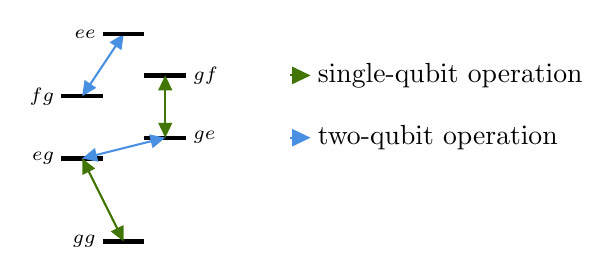
\begin{tikzpicture}[x=0.75pt,y=0.75pt,yscale=-1,xscale=1]
%uncomment if require: \path (0,300); %set diagram left start at 0, and has height of 300

%Straight Lines [id:da9559663622579351] 
\draw [line width=1.5]    (100,100) -- (120,100) ;
%Straight Lines [id:da38130444644691297] 
\draw [line width=1.5]    (140,90) -- (160,90) ;
%Straight Lines [id:da2359488638530448] 
\draw [line width=1.5]    (100,130) -- (120,130) ;
%Straight Lines [id:da3841009239924672] 
\draw [line width=1.5]    (120,170) -- (140,170) ;
%Straight Lines [id:da5788606590900368] 
\draw [line width=1.5]    (140,120) -- (160,120) ;
%Straight Lines [id:da9477773949836692] 
\draw [color={rgb, 255:red, 65; green, 117; blue, 5 }  ,draw opacity=1 ]   (111.34,132.68) -- (128.66,167.32) ;
\draw [shift={(130,170)}, rotate = 243.43] [fill={rgb, 255:red, 65; green, 117; blue, 5 }  ,fill opacity=1 ][line width=0.08]  [draw opacity=0] (7.14,-3.43) -- (0,0) -- (7.14,3.43) -- cycle    ;
\draw [shift={(110,130)}, rotate = 63.43] [fill={rgb, 255:red, 65; green, 117; blue, 5 }  ,fill opacity=1 ][line width=0.08]  [draw opacity=0] (7.14,-3.43) -- (0,0) -- (7.14,3.43) -- cycle    ;
%Straight Lines [id:da6539701699881647] 
\draw [color={rgb, 255:red, 74; green, 144; blue, 226 }  ,draw opacity=1 ]   (128.34,72.5) -- (111.66,97.5) ;
\draw [shift={(110,100)}, rotate = 303.69] [fill={rgb, 255:red, 74; green, 144; blue, 226 }  ,fill opacity=1 ][line width=0.08]  [draw opacity=0] (7.14,-3.43) -- (0,0) -- (7.14,3.43) -- cycle    ;
\draw [shift={(130,70)}, rotate = 123.69] [fill={rgb, 255:red, 74; green, 144; blue, 226 }  ,fill opacity=1 ][line width=0.08]  [draw opacity=0] (7.14,-3.43) -- (0,0) -- (7.14,3.43) -- cycle    ;
%Straight Lines [id:da6430626577491835] 
\draw [color={rgb, 255:red, 65; green, 117; blue, 5 }  ,draw opacity=1 ]   (210,90) -- (217,90) ;
\draw [shift={(220,90)}, rotate = 180] [fill={rgb, 255:red, 65; green, 117; blue, 5 }  ,fill opacity=1 ][line width=0.08]  [draw opacity=0] (8.93,-4.29) -- (0,0) -- (8.93,4.29) -- cycle    ;
%Straight Lines [id:da593444231277527] 
\draw [color={rgb, 255:red, 74; green, 144; blue, 226 }  ,draw opacity=1 ]   (210,120) -- (217,120) ;
\draw [shift={(220,120)}, rotate = 180] [fill={rgb, 255:red, 74; green, 144; blue, 226 }  ,fill opacity=1 ][line width=0.08]  [draw opacity=0] (8.93,-4.29) -- (0,0) -- (8.93,4.29) -- cycle    ;
%Straight Lines [id:da04551771823475548] 
\draw [line width=1.5]    (120,70) -- (140,70) ;
%Straight Lines [id:da8060801042251682] 
\draw [color={rgb, 255:red, 65; green, 117; blue, 5 }  ,draw opacity=1 ]   (150,93) -- (150,117) ;
\draw [shift={(150,120)}, rotate = 270] [fill={rgb, 255:red, 65; green, 117; blue, 5 }  ,fill opacity=1 ][line width=0.08]  [draw opacity=0] (7.14,-3.43) -- (0,0) -- (7.14,3.43) -- cycle    ;
\draw [shift={(150,90)}, rotate = 90] [fill={rgb, 255:red, 65; green, 117; blue, 5 }  ,fill opacity=1 ][line width=0.08]  [draw opacity=0] (7.14,-3.43) -- (0,0) -- (7.14,3.43) -- cycle    ;
%Straight Lines [id:da40683969551339827] 
\draw [color={rgb, 255:red, 74; green, 144; blue, 226 }  ,draw opacity=1 ]   (112.91,129.27) -- (147.09,120.73) ;
\draw [shift={(150,120)}, rotate = 165.96] [fill={rgb, 255:red, 74; green, 144; blue, 226 }  ,fill opacity=1 ][line width=0.08]  [draw opacity=0] (7.14,-3.43) -- (0,0) -- (7.14,3.43) -- cycle    ;
\draw [shift={(110,130)}, rotate = 345.96] [fill={rgb, 255:red, 74; green, 144; blue, 226 }  ,fill opacity=1 ][line width=0.08]  [draw opacity=0] (7.14,-3.43) -- (0,0) -- (7.14,3.43) -- cycle    ;

% Text Node
\draw (98,100) node [anchor=east] [inner sep=0.75pt]  [font=\scriptsize]  {$fg$};
% Text Node
\draw (98,130) node [anchor=east] [inner sep=0.75pt]  [font=\scriptsize]  {$eg$};
% Text Node
\draw (118,170) node [anchor=east] [inner sep=0.75pt]  [font=\scriptsize]  {$gg$};
% Text Node
\draw (162,90) node [anchor=west] [inner sep=0.75pt]  [font=\scriptsize]  {$gf$};
% Text Node
\draw (162,120) node [anchor=west] [inner sep=0.75pt]  [font=\scriptsize]  {$ge$};
% Text Node
\draw (222,90) node [anchor=west] [inner sep=0.75pt]   [align=left] {single-qubit operation};
% Text Node
\draw (222,120) node [anchor=west] [inner sep=0.75pt]   [align=left] {two-qubit operation};
% Text Node
\draw (118,70) node [anchor=east] [inner sep=0.75pt]  [font=\scriptsize]  {$ee$};


\end{tikzpicture}
    \vspace{-1cm}
    \caption{Level diagram of storage-storage interaction}
    \label{fig:SS_level}
\end{figure}

In \cref{fig:SS_level}, the energy levels of the two-qubits system is shown, together with some single- and two-qubit gates that we can run on them.

\subsection{CZ}

The unitary matrix representing a controlled-phase gate, or CZ, is
\begin{equation}
    U_{\text{CZ}} = 
    \begin{pmatrix}
    1 & 0 & 0 & 0 \\
    0 & 1 & 0 & 0 \\
    0 & 0 & 1 & 0 \\
    0 & 0 & 0 & -1 \\
\end{pmatrix}.
\end{equation}

It performs the operation
\begin{equation}
    (\alpha \ket{gg} + \beta \ket{ge} + \gamma \ket{eg} + \delta \ket{ee})_{\text{S}_1 \text{S}_2} \xrightarrow{U_{\text{CZ}}}
    (\alpha \ket{gg} + \beta \ket{ge} + \gamma \ket{eg} - \delta \ket{ee})_{\text{S}_1 \text{S}_2} . 
\end{equation}

The operational sequence on our device involves transferring population between the states $\ket{ee}$ and $\ket{fg}$ within the S-S system.
After a $2\pi$ rotation, the population returns to the $\ket{ee}$ state, but with an acquired phase of $\pi$ (see \cref{fig:SS_CZ}), effectively implementing a CZ gate.

\begin{figure}
    \centering
    

\tikzset{every picture/.style={line width=0.75pt}} %set default line width to 0.75pt        

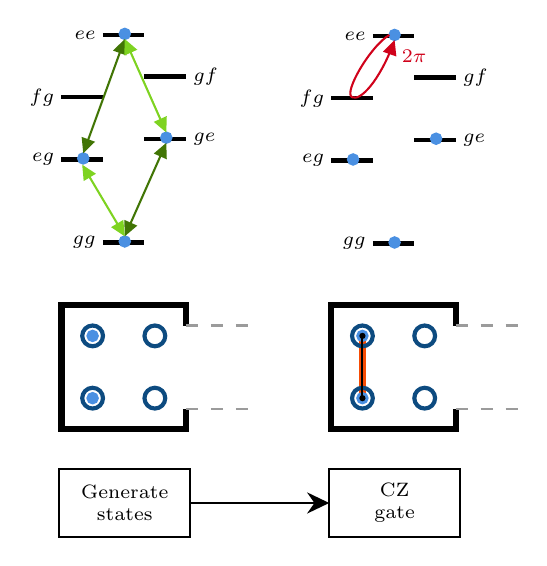
\begin{tikzpicture}[x=0.75pt,y=0.75pt,yscale=-1,xscale=1]
%uncomment if require: \path (0,369); %set diagram left start at 0, and has height of 369

%Straight Lines [id:da14238319538466393] 
\draw [color={rgb, 255:red, 246; green, 76; blue, 4 }  ,draw opacity=1 ][line width=2.25]    (185,215) -- (185,245) ;
%Shape: Circle [id:dp6131452055369363] 
\draw  [color={rgb, 255:red, 13; green, 75; blue, 128 }  ,draw opacity=1 ][line width=1.5]  (180,215) .. controls (180,212.24) and (182.24,210) .. (185,210) .. controls (187.76,210) and (190,212.24) .. (190,215) .. controls (190,217.76) and (187.76,220) .. (185,220) .. controls (182.24,220) and (180,217.76) .. (180,215) -- cycle ;
%Shape: Circle [id:dp044196496820445685] 
\draw  [color={rgb, 255:red, 13; green, 75; blue, 128 }  ,draw opacity=1 ][line width=1.5]  (180,245) .. controls (180,242.24) and (182.24,240) .. (185,240) .. controls (187.76,240) and (190,242.24) .. (190,245) .. controls (190,247.76) and (187.76,250) .. (185,250) .. controls (182.24,250) and (180,247.76) .. (180,245) -- cycle ;
%Shape: Circle [id:dp5885154746260259] 
\draw  [color={rgb, 255:red, 13; green, 75; blue, 128 }  ,draw opacity=1 ][line width=1.5]  (210,245) .. controls (210,242.24) and (212.24,240) .. (215,240) .. controls (217.76,240) and (220,242.24) .. (220,245) .. controls (220,247.76) and (217.76,250) .. (215,250) .. controls (212.24,250) and (210,247.76) .. (210,245) -- cycle ;
%Shape: Circle [id:dp7469388514126467] 
\draw  [color={rgb, 255:red, 13; green, 75; blue, 128 }  ,draw opacity=1 ][line width=1.5]  (210,215) .. controls (210,212.24) and (212.24,210) .. (215,210) .. controls (217.76,210) and (220,212.24) .. (220,215) .. controls (220,217.76) and (217.76,220) .. (215,220) .. controls (212.24,220) and (210,217.76) .. (210,215) -- cycle ;
%Shape: Square [id:dp8509793592974496] 
\draw  [line width=2.25]  (170,200) -- (230,200) -- (230,260) -- (170,260) -- cycle ;
%Straight Lines [id:da12483962352096123] 
\draw [color={rgb, 255:red, 255; green, 255; blue, 255 }  ,draw opacity=1 ][line width=3]    (230,210) -- (230,250) ;

%Shape: Circle [id:dp2946136793659927] 
\draw  [color={rgb, 255:red, 74; green, 144; blue, 226 }  ,draw opacity=1 ][fill={rgb, 255:red, 74; green, 144; blue, 226 }  ,fill opacity=1 ] (182.5,215) .. controls (182.5,213.62) and (183.62,212.5) .. (185,212.5) .. controls (186.38,212.5) and (187.5,213.62) .. (187.5,215) .. controls (187.5,216.38) and (186.38,217.5) .. (185,217.5) .. controls (183.62,217.5) and (182.5,216.38) .. (182.5,215) -- cycle ;
%Straight Lines [id:da5174133920036248] 
\draw [color={rgb, 255:red, 155; green, 155; blue, 155 }  ,draw opacity=1 ] [dash pattern={on 4.5pt off 4.5pt}]  (230,210) -- (260,210) ;
%Straight Lines [id:da26746057224200814] 
\draw [color={rgb, 255:red, 155; green, 155; blue, 155 }  ,draw opacity=1 ] [dash pattern={on 4.5pt off 4.5pt}]  (230,250) -- (260,250) ;
%Shape: Circle [id:dp9726522957124347] 
\draw  [color={rgb, 255:red, 13; green, 75; blue, 128 }  ,draw opacity=1 ][line width=1.5]  (50,215) .. controls (50,212.24) and (52.24,210) .. (55,210) .. controls (57.76,210) and (60,212.24) .. (60,215) .. controls (60,217.76) and (57.76,220) .. (55,220) .. controls (52.24,220) and (50,217.76) .. (50,215) -- cycle ;
%Shape: Circle [id:dp5051693054900083] 
\draw  [color={rgb, 255:red, 13; green, 75; blue, 128 }  ,draw opacity=1 ][line width=1.5]  (50,245) .. controls (50,242.24) and (52.24,240) .. (55,240) .. controls (57.76,240) and (60,242.24) .. (60,245) .. controls (60,247.76) and (57.76,250) .. (55,250) .. controls (52.24,250) and (50,247.76) .. (50,245) -- cycle ;
%Shape: Circle [id:dp6033756962982088] 
\draw  [color={rgb, 255:red, 13; green, 75; blue, 128 }  ,draw opacity=1 ][line width=1.5]  (80,245) .. controls (80,242.24) and (82.24,240) .. (85,240) .. controls (87.76,240) and (90,242.24) .. (90,245) .. controls (90,247.76) and (87.76,250) .. (85,250) .. controls (82.24,250) and (80,247.76) .. (80,245) -- cycle ;
%Shape: Circle [id:dp651180579558279] 
\draw  [color={rgb, 255:red, 13; green, 75; blue, 128 }  ,draw opacity=1 ][line width=1.5]  (80,215) .. controls (80,212.24) and (82.24,210) .. (85,210) .. controls (87.76,210) and (90,212.24) .. (90,215) .. controls (90,217.76) and (87.76,220) .. (85,220) .. controls (82.24,220) and (80,217.76) .. (80,215) -- cycle ;
%Shape: Square [id:dp8220576054517261] 
\draw  [line width=2.25]  (40,200) -- (100,200) -- (100,260) -- (40,260) -- cycle ;
%Straight Lines [id:da3250679662921139] 
\draw [color={rgb, 255:red, 255; green, 255; blue, 255 }  ,draw opacity=1 ][line width=3]    (100,210) -- (100,250) ;

%Shape: Circle [id:dp1764454757841779] 
\draw  [color={rgb, 255:red, 74; green, 144; blue, 226 }  ,draw opacity=1 ][fill={rgb, 255:red, 74; green, 144; blue, 226 }  ,fill opacity=1 ] (52.5,215) .. controls (52.5,213.62) and (53.62,212.5) .. (55,212.5) .. controls (56.38,212.5) and (57.5,213.62) .. (57.5,215) .. controls (57.5,216.38) and (56.38,217.5) .. (55,217.5) .. controls (53.62,217.5) and (52.5,216.38) .. (52.5,215) -- cycle ;
%Straight Lines [id:da9570390374106923] 
\draw [color={rgb, 255:red, 155; green, 155; blue, 155 }  ,draw opacity=1 ] [dash pattern={on 4.5pt off 4.5pt}]  (100,210) -- (130,210) ;
%Straight Lines [id:da8355397813605424] 
\draw [color={rgb, 255:red, 155; green, 155; blue, 155 }  ,draw opacity=1 ] [dash pattern={on 4.5pt off 4.5pt}]  (100,250) -- (130,250) ;
%Straight Lines [id:da605984992083237] 
\draw [line width=1.5]    (40,100) -- (60,100) ;
%Straight Lines [id:da38731851189389244] 
\draw [line width=1.5]    (80,90) -- (100,90) ;
%Straight Lines [id:da4898165874704924] 
\draw [line width=1.5]    (40,130) -- (60,130) ;
%Straight Lines [id:da24826706546268984] 
\draw [line width=1.5]    (60,170) -- (80,170) ;
%Straight Lines [id:da43859897810303505] 
\draw [line width=1.5]    (80,120) -- (100,120) ;
%Straight Lines [id:da33344037757379863] 
\draw [line width=1.5]    (60,70) -- (80,70) ;
%Shape: Circle [id:dp7629931524746876] 
\draw  [color={rgb, 255:red, 74; green, 144; blue, 226 }  ,draw opacity=1 ][fill={rgb, 255:red, 74; green, 144; blue, 226 }  ,fill opacity=1 ] (68,169.5) .. controls (68,168.12) and (69.12,167) .. (70.5,167) .. controls (71.88,167) and (73,168.12) .. (73,169.5) .. controls (73,170.88) and (71.88,172) .. (70.5,172) .. controls (69.12,172) and (68,170.88) .. (68,169.5) -- cycle ;
%Shape: Circle [id:dp9222004689061901] 
\draw  [color={rgb, 255:red, 74; green, 144; blue, 226 }  ,draw opacity=1 ][fill={rgb, 255:red, 74; green, 144; blue, 226 }  ,fill opacity=1 ] (48,129.5) .. controls (48,128.12) and (49.12,127) .. (50.5,127) .. controls (51.88,127) and (53,128.12) .. (53,129.5) .. controls (53,130.88) and (51.88,132) .. (50.5,132) .. controls (49.12,132) and (48,130.88) .. (48,129.5) -- cycle ;
%Shape: Circle [id:dp5632081381008429] 
\draw  [color={rgb, 255:red, 74; green, 144; blue, 226 }  ,draw opacity=1 ][fill={rgb, 255:red, 74; green, 144; blue, 226 }  ,fill opacity=1 ] (88,119.5) .. controls (88,118.12) and (89.12,117) .. (90.5,117) .. controls (91.88,117) and (93,118.12) .. (93,119.5) .. controls (93,120.88) and (91.88,122) .. (90.5,122) .. controls (89.12,122) and (88,120.88) .. (88,119.5) -- cycle ;
%Shape: Circle [id:dp023555240322724158] 
\draw  [color={rgb, 255:red, 74; green, 144; blue, 226 }  ,draw opacity=1 ][fill={rgb, 255:red, 74; green, 144; blue, 226 }  ,fill opacity=1 ] (68,69.5) .. controls (68,68.12) and (69.12,67) .. (70.5,67) .. controls (71.88,67) and (73,68.12) .. (73,69.5) .. controls (73,70.88) and (71.88,72) .. (70.5,72) .. controls (69.12,72) and (68,70.88) .. (68,69.5) -- cycle ;
%Straight Lines [id:da4406201929591368] 
\draw [color={rgb, 255:red, 65; green, 117; blue, 5 }  ,draw opacity=1 ]   (89.28,124.74) -- (71.72,164.26) ;
\draw [shift={(70.5,167)}, rotate = 293.96] [fill={rgb, 255:red, 65; green, 117; blue, 5 }  ,fill opacity=1 ][line width=0.08]  [draw opacity=0] (7.14,-3.43) -- (0,0) -- (7.14,3.43) -- cycle    ;
\draw [shift={(90.5,122)}, rotate = 113.96] [fill={rgb, 255:red, 65; green, 117; blue, 5 }  ,fill opacity=1 ][line width=0.08]  [draw opacity=0] (7.14,-3.43) -- (0,0) -- (7.14,3.43) -- cycle    ;
%Straight Lines [id:da9819884495181663] 
\draw [color={rgb, 255:red, 65; green, 117; blue, 5 }  ,draw opacity=1 ]   (69.47,74.82) -- (51.53,124.18) ;
\draw [shift={(50.5,127)}, rotate = 289.98] [fill={rgb, 255:red, 65; green, 117; blue, 5 }  ,fill opacity=1 ][line width=0.08]  [draw opacity=0] (7.14,-3.43) -- (0,0) -- (7.14,3.43) -- cycle    ;
\draw [shift={(70.5,72)}, rotate = 109.98] [fill={rgb, 255:red, 65; green, 117; blue, 5 }  ,fill opacity=1 ][line width=0.08]  [draw opacity=0] (7.14,-3.43) -- (0,0) -- (7.14,3.43) -- cycle    ;
%Straight Lines [id:da9796916063314295] 
\draw [color={rgb, 255:red, 126; green, 211; blue, 33 }  ,draw opacity=1 ]   (71.72,74.74) -- (89.28,114.26) ;
\draw [shift={(90.5,117)}, rotate = 246.04] [fill={rgb, 255:red, 126; green, 211; blue, 33 }  ,fill opacity=1 ][line width=0.08]  [draw opacity=0] (7.14,-3.43) -- (0,0) -- (7.14,3.43) -- cycle    ;
\draw [shift={(70.5,72)}, rotate = 66.04] [fill={rgb, 255:red, 126; green, 211; blue, 33 }  ,fill opacity=1 ][line width=0.08]  [draw opacity=0] (7.14,-3.43) -- (0,0) -- (7.14,3.43) -- cycle    ;
%Straight Lines [id:da25683659760281263] 
\draw [color={rgb, 255:red, 126; green, 211; blue, 33 }  ,draw opacity=1 ]   (51.53,135.08) -- (68.97,164.42) ;
\draw [shift={(70.5,167)}, rotate = 239.28] [fill={rgb, 255:red, 126; green, 211; blue, 33 }  ,fill opacity=1 ][line width=0.08]  [draw opacity=0] (7.14,-3.43) -- (0,0) -- (7.14,3.43) -- cycle    ;
\draw [shift={(50,132.5)}, rotate = 59.28] [fill={rgb, 255:red, 126; green, 211; blue, 33 }  ,fill opacity=1 ][line width=0.08]  [draw opacity=0] (7.14,-3.43) -- (0,0) -- (7.14,3.43) -- cycle    ;
%Straight Lines [id:da9637012758897168] 
\draw [line width=1.5]    (170,100.5) -- (190,100.5) ;
%Straight Lines [id:da8684535686248622] 
\draw [line width=1.5]    (210,90.5) -- (230,90.5) ;
%Straight Lines [id:da17021177110230912] 
\draw [line width=1.5]    (170,130.5) -- (190,130.5) ;
%Straight Lines [id:da7796352034758786] 
\draw [line width=1.5]    (190,170.5) -- (210,170.5) ;
%Straight Lines [id:da41159550798158584] 
\draw [line width=1.5]    (210,120.5) -- (230,120.5) ;
%Straight Lines [id:da7308144564661493] 
\draw [line width=1.5]    (190,70.5) -- (210,70.5) ;
%Shape: Circle [id:dp8827634585194027] 
\draw  [color={rgb, 255:red, 74; green, 144; blue, 226 }  ,draw opacity=1 ][fill={rgb, 255:red, 74; green, 144; blue, 226 }  ,fill opacity=1 ] (198,170) .. controls (198,168.62) and (199.12,167.5) .. (200.5,167.5) .. controls (201.88,167.5) and (203,168.62) .. (203,170) .. controls (203,171.38) and (201.88,172.5) .. (200.5,172.5) .. controls (199.12,172.5) and (198,171.38) .. (198,170) -- cycle ;
%Shape: Circle [id:dp12686587985832598] 
\draw  [color={rgb, 255:red, 74; green, 144; blue, 226 }  ,draw opacity=1 ][fill={rgb, 255:red, 74; green, 144; blue, 226 }  ,fill opacity=1 ] (178,130) .. controls (178,128.62) and (179.12,127.5) .. (180.5,127.5) .. controls (181.88,127.5) and (183,128.62) .. (183,130) .. controls (183,131.38) and (181.88,132.5) .. (180.5,132.5) .. controls (179.12,132.5) and (178,131.38) .. (178,130) -- cycle ;
%Shape: Circle [id:dp6893004504301061] 
\draw  [color={rgb, 255:red, 74; green, 144; blue, 226 }  ,draw opacity=1 ][fill={rgb, 255:red, 74; green, 144; blue, 226 }  ,fill opacity=1 ] (218,120) .. controls (218,118.62) and (219.12,117.5) .. (220.5,117.5) .. controls (221.88,117.5) and (223,118.62) .. (223,120) .. controls (223,121.38) and (221.88,122.5) .. (220.5,122.5) .. controls (219.12,122.5) and (218,121.38) .. (218,120) -- cycle ;
%Shape: Circle [id:dp6629315947880386] 
\draw  [color={rgb, 255:red, 74; green, 144; blue, 226 }  ,draw opacity=1 ][fill={rgb, 255:red, 74; green, 144; blue, 226 }  ,fill opacity=1 ] (198,70) .. controls (198,68.62) and (199.12,67.5) .. (200.5,67.5) .. controls (201.88,67.5) and (203,68.62) .. (203,70) .. controls (203,71.38) and (201.88,72.5) .. (200.5,72.5) .. controls (199.12,72.5) and (198,71.38) .. (198,70) -- cycle ;
%Curve Lines [id:da5178021924441131] 
\draw [color={rgb, 255:red, 208; green, 2; blue, 27 }  ,draw opacity=1 ]   (198,70) .. controls (189,75.17) and (175.67,97.83) .. (180,100) .. controls (184.12,102.06) and (193.05,91.93) .. (199.5,75.2) ;
\draw [shift={(200.5,72.5)}, rotate = 109.52] [fill={rgb, 255:red, 208; green, 2; blue, 27 }  ,fill opacity=1 ][line width=0.08]  [draw opacity=0] (7.14,-3.43) -- (0,0) -- (7.14,3.43) -- cycle    ;
%Shape: Circle [id:dp26197554740985884] 
\draw  [color={rgb, 255:red, 74; green, 144; blue, 226 }  ,draw opacity=1 ][fill={rgb, 255:red, 74; green, 144; blue, 226 }  ,fill opacity=1 ] (52.5,245) .. controls (52.5,243.62) and (53.62,242.5) .. (55,242.5) .. controls (56.38,242.5) and (57.5,243.62) .. (57.5,245) .. controls (57.5,246.38) and (56.38,247.5) .. (55,247.5) .. controls (53.62,247.5) and (52.5,246.38) .. (52.5,245) -- cycle ;
%Shape: Circle [id:dp7779633747567205] 
\draw  [color={rgb, 255:red, 74; green, 144; blue, 226 }  ,draw opacity=1 ][fill={rgb, 255:red, 74; green, 144; blue, 226 }  ,fill opacity=1 ] (182.5,245) .. controls (182.5,243.62) and (183.62,242.5) .. (185,242.5) .. controls (186.38,242.5) and (187.5,243.62) .. (187.5,245) .. controls (187.5,246.38) and (186.38,247.5) .. (185,247.5) .. controls (183.62,247.5) and (182.5,246.38) .. (182.5,245) -- cycle ;
%Straight Lines [id:da5417689626607565] 
\draw    (185,215) -- (185,245) ;
%Shape: Circle [id:dp8939955847994656] 
\draw  [draw opacity=0][fill={rgb, 255:red, 0; green, 0; blue, 0 }  ,fill opacity=1 ] (183.5,215) .. controls (183.5,214.17) and (184.17,213.5) .. (185,213.5) .. controls (185.83,213.5) and (186.5,214.17) .. (186.5,215) .. controls (186.5,215.83) and (185.83,216.5) .. (185,216.5) .. controls (184.17,216.5) and (183.5,215.83) .. (183.5,215) -- cycle ;
%Shape: Circle [id:dp5788101040789697] 
\draw  [draw opacity=0][fill={rgb, 255:red, 0; green, 0; blue, 0 }  ,fill opacity=1 ] (183.5,245) .. controls (183.5,244.17) and (184.17,243.5) .. (185,243.5) .. controls (185.83,243.5) and (186.5,244.17) .. (186.5,245) .. controls (186.5,245.83) and (185.83,246.5) .. (185,246.5) .. controls (184.17,246.5) and (183.5,245.83) .. (183.5,245) -- cycle ;

% Text Node
\draw (202.5,75.9) node [anchor=north west][inner sep=0.75pt]  [font=\scriptsize,color={rgb, 255:red, 208; green, 2; blue, 27 }  ,opacity=1 ]  {$2\pi $};
% Text Node
\draw    (169,279) -- (232,279) -- (232,312) -- (169,312) -- cycle  ;
\draw (200.5,295.5) node  [font=\scriptsize] [align=left] {\begin{minipage}[lt]{40.8pt}\setlength\topsep{0pt}
\begin{center}
CZ\\gate
\end{center}

\end{minipage}};
% Text Node
\draw    (39,279) -- (102,279) -- (102,312) -- (39,312) -- cycle  ;
\draw (70.5,295.5) node  [font=\scriptsize] [align=left] {\begin{minipage}[lt]{40.8pt}\setlength\topsep{0pt}
\begin{center}
Generate\\states
\end{center}

\end{minipage}};
% Text Node
\draw (38,100) node [anchor=east] [inner sep=0.75pt]  [font=\scriptsize]  {$fg$};
% Text Node
\draw (38,130) node [anchor=east] [inner sep=0.75pt]  [font=\scriptsize]  {$eg$};
% Text Node
\draw (58,170) node [anchor=east] [inner sep=0.75pt]  [font=\scriptsize]  {$gg$};
% Text Node
\draw (102,90) node [anchor=west] [inner sep=0.75pt]  [font=\scriptsize]  {$gf$};
% Text Node
\draw (102,120) node [anchor=west] [inner sep=0.75pt]  [font=\scriptsize]  {$ge$};
% Text Node
\draw (58,70) node [anchor=east] [inner sep=0.75pt]  [font=\scriptsize]  {$ee$};
% Text Node
\draw (168,100.5) node [anchor=east] [inner sep=0.75pt]  [font=\scriptsize]  {$fg$};
% Text Node
\draw (168,130.5) node [anchor=east] [inner sep=0.75pt]  [font=\scriptsize]  {$eg$};
% Text Node
\draw (188,170.5) node [anchor=east] [inner sep=0.75pt]  [font=\scriptsize]  {$gg$};
% Text Node
\draw (232,90.5) node [anchor=west] [inner sep=0.75pt]  [font=\scriptsize]  {$gf$};
% Text Node
\draw (232,120.5) node [anchor=west] [inner sep=0.75pt]  [font=\scriptsize]  {$ge$};
% Text Node
\draw (188,70.5) node [anchor=east] [inner sep=0.75pt]  [font=\scriptsize]  {$ee$};
% Connection
\draw    (102,295.5) -- (166,295.5) ;
\draw [shift={(169,295.5)}, rotate = 180] [fill={rgb, 255:red, 0; green, 0; blue, 0 }  ][line width=0.08]  [draw opacity=0] (10.72,-5.15) -- (0,0) -- (10.72,5.15) -- (7.12,0) -- cycle    ;

\end{tikzpicture}
    \vspace{-1cm}
    \caption{Protocol for S-S CZ gate}
    \label{fig:SS_CZ}
\end{figure}

\begin{figure}[b]
    \centering
    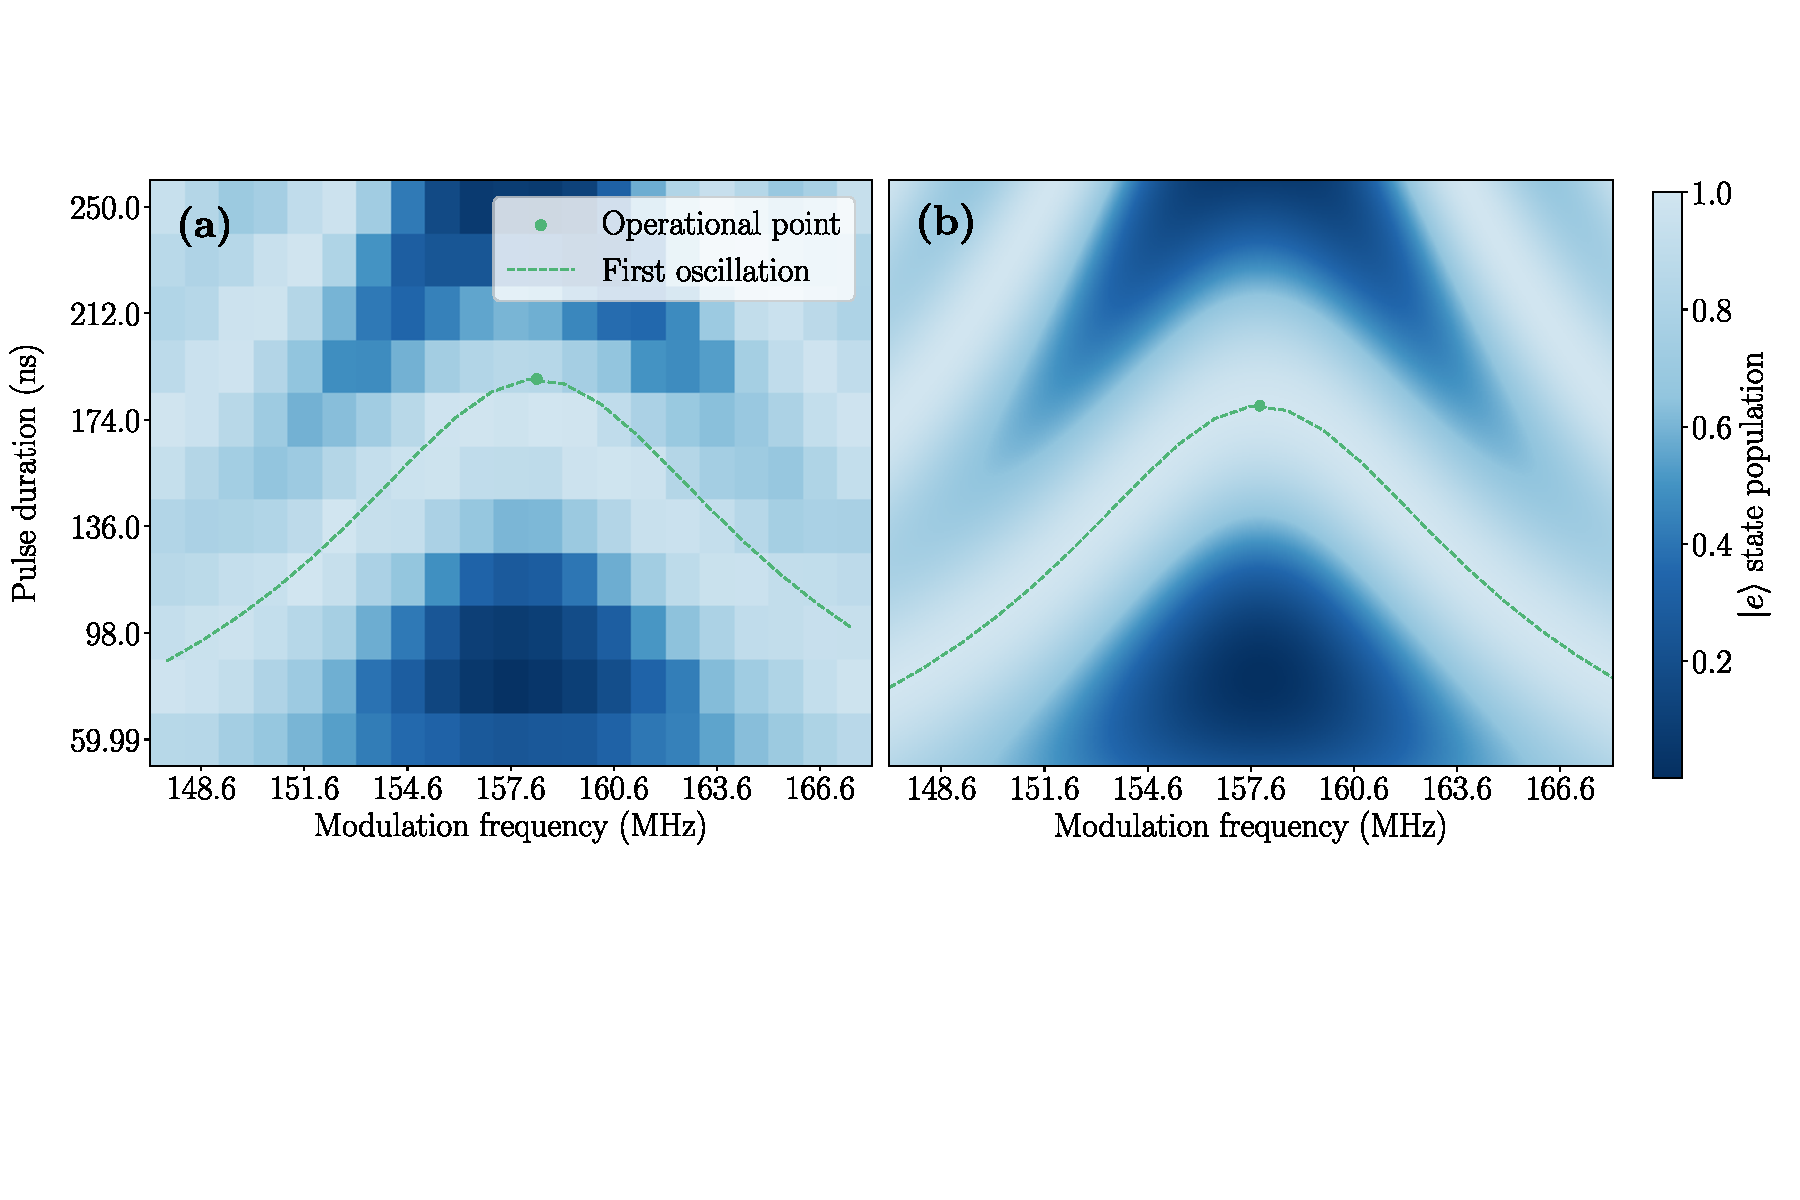
\includegraphics[width=\linewidth]{Images//Chap3/Chevron_b_double.pdf}
    \caption{\textbf{(a)} data of the $eefg$ transition within a storage-storage pair with \textbf{(b)} relative fit}
    \label{fig:Chev_data}
\end{figure}

In this context, it is necessary to calibrate the interaction between the $ee$ and $fg$ energy levels.
For this purpose, we employ the previously derived model, using \cref{eq:chevron} to perform fitting on the data.
Fig.~\ref{fig:Chev_data} shows the data and the respective fit.
It also shows the operational point for implementing the CZ gate.
This operational point is given by
\begin{equation}
    \widetilde{t} = \frac{1}{2 g_0}.
\end{equation}

On \cref{fig:Chev_data} is also depicted the first oscillation period as a function of the detuning $\delta$, given by
\begin{equation}
    t = \frac{1}{\sqrt{4 g_0^2 + \delta^2}} . 
\end{equation}